\chapter{Floating-point representations}
\label{ch:background}
Among the different methods to represent the set of real numbers in computers,
floating-points are a commonly adopted format.
This chapter discusses some fundamental definitions and basic notions on
floating-points, briefly describes the IEEE~754~\cite{ieee754_2008-ev} data format, and 
explains the sources of errors in floating-point arithmethic and their consequences.
The content in this chapter is based on~\cite{Muller2018-zm}.

\section{Definitions and basic notions}
A floating-point format is defined with four intergers:
\begin{itemize}
	\item A \textit{radix} (or \textit{Base}) $B \ge 2$.
	\item A \textit{precision} $p \ge 2$ which approximately represents the number of significant digits for the format.
	\item Two exponent $e_{min}$ and $e_{max}$ that bound the range of value represent by the format. In practice, $e_{min} \le 0 \le e_{max}$.
\end{itemize}

A floating-point number in such a format is a number $x$ that can be represented by a pair $(M,e)$, such that
\begin{equation}
	x = M \cdot B^{e-p+1}
\end{equation}
where
\begin{itemize}
	\item $M$ is an integer such that $|M| \le B^{p}-1$. It is called the \textit{integral significand} of x\tristan{or the mantissa?}.\MD{The integral significand is different from the normal significand. i.e. it is not normalized using $m = |M| \cdot B^{1-p}$, where $m$ would be the mantissa.}
	\item $e$ is an integer such that $e_{min} \le e \le e_{max}$. It is called the \textit{exponent} of x.
\end{itemize}
The representation of a number using a pair $(M, e)$ is not unique.
The set of all such representation is called a \textit{cohort}.
It is often desirable to have a unique representation; i.e. \tristan{fix syntax} called \textit{normalized representation}.
This simplifies the expression of error bounds and the implementation.
It can be achieved, for example, by always representing numbers using the minimum possible exponent.
Floating-points are often categorized into \textit{normal} and \textit{subnormal} (also called \textit{denormal}) numbers.
In radix 2, the first digits of a siginificand is 1 for normal numbers and 0 for subnormal ones.
\HL{This deterministic information enables an encoding strategy known as \textit{hidden bit convention} (described in Section~{\ref{sc:ieee754}}),
which avoids storing the most significant bit while preserving the same precision.}
Moreover, the availability of subnormal numbers allows for \textit{gradual underflow},
which helps implementing numerically stable code. \tristan{Add a sentence to explain what it is.}
				
A common way to define the error introduced by a floating-point arithmetic
operation is the \textit{unit in the last place (ulp)}.
\HL{Given a number x, represented as a floating-point,} $ulp(x)$ is defined as the distance between the two closest distinct
floating-point numbers $a$ and $b$, such that \HL{$a \le x \le b$} and $a \neq b$.
\HL{In other words, one ulp is equal to $B^{e-p+1}$.}

A function is \textit{correctly rounded} when its results are always rounded the 
same way as if it used infinite precision and range.
In other words, a function is correctly rounded when its error is within $0.5$ ulp.
When a function cannot guarantee correct rounding and always rounds a number $y$
using one of \textit{round-up} or \textit{round-down} function, it is said to be \textit{faithful}.
Correctly rounded functions are always faithful.
One must keep in mind that even if a function is correctly rounded, there is
still loss of information if the number cannot be represented exactly in the
floating-point format.
				
With floating-point arithmetic, some properties from real number arithmetic are lost while other ones remain.
Correctly rounded arithmetic operations remain commutative with addition and multiplication.
\tristan{How about incorrectly rounded functions?}
However, associativity and distributivity no longer apply.
If not cautious about this, it can result in drastic errors. 

\tristan{content is great but you should really use a spellchecker!}
				
				
\section{IEEE~754 Binary format}
\label{sc:ieee754}
Since the beginning of computers, there have been multiple proposed solutions to represent floating-point numbers.
In this section, we limit our focus to the IEEE~754-2008 format, shortened to IEEE~754, as it is largely adopted in hardware.
The IEEE~754 format describes a standard for radix 2 and 10, Binary and Decimal, respectively.
We limit our scope to the Binary data type since Decimal is mostly used in financial applications which are outside the scope of our research.
				
IEEE~754 defines three basic formats for Binary: 32, 64, and 128 bits.
It also defines a suggested format for 16 bits.
In all those formats, a set precision is defined as well as a range for the exponent values of $e_{min} = 1 - e_{max}$.
Table~\ref{table:IEEE754-binary-parameters} shows the precision and exponent parameters for each format. 
				
\begin{table}[h]
	\centering
	\begin{tabular}{|c|r|r|r|r|}
		\hline
		Name &
		binary16 &
		\begin{tabular}[c]{@{}r@{}}binary32\\ (basic)\end{tabular} &
		\begin{tabular}[c]{@{}r@{}}binary64\\ (basic)\end{tabular} &
		\begin{tabular}[c]{@{}r@{}}binary128\\ (basic)\end{tabular} \\ \hline
		Former name &
		N/A &
		\begin{tabular}[c]{@{}r@{}}single\\ precision\end{tabular} &
		\begin{tabular}[c]{@{}r@{}}double\\ precision\end{tabular} &
		N/A \\ \hline
		p         & 11  & 24   & 53    & 113    \\ \hline
		$e_{max}$ & +15 & +127 & +1023 & +16383 \\ \hline
		$e_{min}$ & -14 & -126 & -1022 & -16382 \\ \hline
	\end{tabular}
	\caption{Parameters for the binary formats defined by IEEE~754-2008}
	\label{table:IEEE754-binary-parameters}
\end{table}
				
For some applications, the defined formats might not offer enough precision.
The IEEE~754 standard defines an extended precision format for width above 128 bits.
Table~\ref{table:IEEE754-extended-parameters} describes the parameters for the extended precision format \tristan{context on extended precision is lacking, what are these parameters?}.
% TODO decide if that should be kept. If so, add the description of the variables from the tables in the text.
Where $t$ is the trailing significant, $w$ is the width of the exponent field, and $b$ is the exponent bias.
\begin{table}[h]
	\centering
	\begin{tabular}{|l|l|}
		\hline
		\multicolumn{1}{|c|}{Parameter} & \multicolumn{1}{c|}{\begin{tabular}[c]{@{}c@{}}Binary$k$ format \\ ($k$ is a multiple of 32)\end{tabular}} \\ \hline
		$k$                             & $\ge 128$                                                       \\ \hline
		$p$                             & $k-\lfloor4\log_2(k)\rceil+13$                                  \\ \hline
		$t$                             & $p-1$                                                           \\ \hline
		$w$                             & $k-t-1$                                                         \\ \hline
		$e_{max}$                       & $2^{w-1}-1$                                                     \\ \hline
		$e_{min}$                       & $1 - e_{max}$                                                   \\ \hline
		$b$                             & $e_{max}$                                                       \\ \hline
	\end{tabular}
	\caption{Parameters for the extended precision binary formats defined by IEEE~754-2008}
	\label{table:IEEE754-extended-parameters}
\end{table}
				
The IEEE~754 binary format is encoded using a sign, exponent, and trailing significand.
Figure~\ref{fig:IEEE754-binary-encoding} depicts the encoding scheme for the formats, 
where $S$ is the sign bit, $E$ are the bits for the exponent, and $T$ are the bits for the trailing significand.
In radix 2, the leftmost bit for subnormal numbers is always 0 while normal numbers is 1.
The IEEE~754 binary format uses this property by not storing the leftmost bit of the significand without loss of precision.
This is done by using special encoding values in the exponent field to distinguish the normal and subnormal numbers.
\HL{This is known has the \textit{hidden bit convention}.}
Similar strategies are employed to represent $\pm 0$, $\pm \inf$, and NaN values.
Table~\ref{table:IEEE754-binary-encoding} shows the different encoding used to represent those values.
				
\begin{figure}[h]
	\centering
	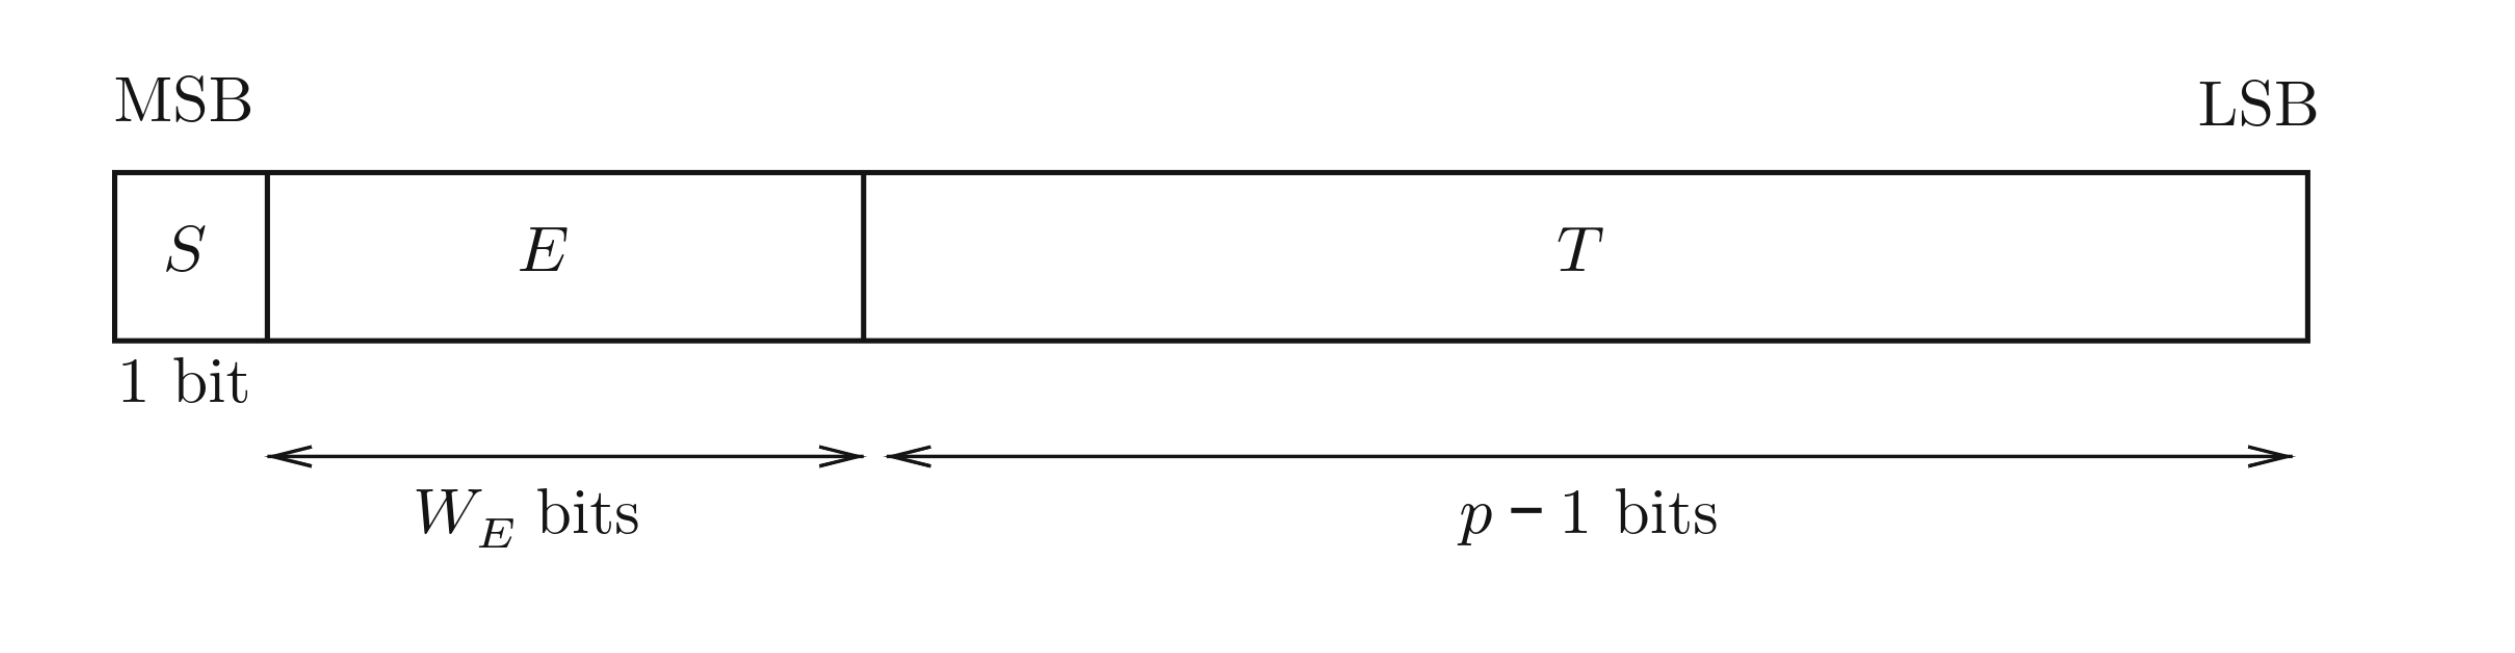
\includegraphics[width=\textwidth]{ieee754_binary_encoding.png}
	\caption{Encoding for the IEEE~754 binary floating-point formats}
	\label{fig:IEEE754-binary-encoding}
\end{figure}
				
\begin{table}[b]
	\centering
	\begin{tabular}{|l|c|c|}
		\hline
		Biased exponent $N_{e}$ &   
		% start 2nd col title
		\begin{tabular} 
		[c]{@{}c@{}}Trailing \\
		significand \\
		$t_{1}t_{2}\cdots t_{p-1}$
	\end{tabular} &
	% end 2nd col title
	Value represented \\ \hline
	$111\cdots1_{2}$      & $\ne 000\cdots 0_{2}$    & NaN                                                          \\ \hline
	$111\cdots1_{2}$      & $\quad 000\cdots 0_{2}$  & $(-1)^{s}\times\inf$                                         \\ \hline
	$000\cdots0_{2}$      & $\quad 000\cdots 0_{2}$  & $(-1)^{s}\times 0$                                           \\ \hline
	$000\cdots0_{2}$      & $\ne 000\cdots 0_{2}$    & $(-1)^{s}\times 0.t_{1}t_{2}\cdots t_{p-1}\times2^{e_{min}}$ \\ \hline
	$0<N_{e}<2^{W_{E}}-1$ & any                      & $(-1)^{s}\times 1.t_{1}t_{2}\cdots t_{p-1}\times2^{N_{e}-b}$ \\ \hline
	\end{tabular}
	\caption{Encoding to represent special values in the binary formats defined by IEEE~754-2008}
	\label{table:IEEE754-binary-encoding}
\end{table}
				
Representing the set of real numbers in a finite space is impossible; instead approximation is required.
The IEEE~754 formats have specified standards regarding rounding of inexact floating-points.
The following arithmetic functions are required to be correctly rounded: addition, subtraction, multiplication, division, and fused multiply-add (FMA).
The square root function and conversion between supported formats also need to be correctly rounded.
Additionally, the standard recommends a list of functions to be correctly rounded. % TODO add reference to list of function (See page 79 of FP handbook)
% TODO Be more specific that this is for IEEE~754 when talking about correctly rounded function. Otherwise it can be confusing. Remove passive voice
There are three directed rounding attributes:
\begin{itemize}
	\item \textit{roundTowardPositive} $RD(x)$ rounds to the largest floating-point less than or equal to $x$.
	\item \textit{roundTowardNegative} $RU(x)$ rounds to the smallest floating-point greater than or equal to $x$.
	\item \textit{roundTowardZero} $RZ(x)$ rounds using $RD(x)$ if $x \ge 0$ or $RU(X)$ if $x \le 0$.
\end{itemize}
There are also two attributes for rounding to nearest, when a floating-point is exactly between two exact representations:
\begin{itemize}
	\item \textit{roundTiesToEven} $RN_{even}(x)$ rounds to the exact representation whose least significant bit is even.
	\item \textit{roundTiesToAway} $RN_{away}(x)$ rounds to the exact representation whose magnitude is the largest.
\end{itemize}
The standard for the binary formats requires the implementation of all three directed rounding and \textit{roundTiesToEven}.
				
While not a basic format, binary16 is starting to receive more attention and support as it is increasingly being used for computing application.
For example, it was found that some convolutional neural networks (CNN) perform well with binary16; and even with a  of only 8 bits \HL{{\cite{Muller2018-zm}}}.
Moreover, while most GPUs support only binary32 and binary64, more recent GPU architectures also support the binary16 format.
				
\section{Sources of error}
% TODO
% Merge with the section: defintion & basic notions.
% 1 page
\begin{comment}
- rounding & double rounding
- cancellation
- overflow & underflow
- accumulation
- swamping

%  Ask Yohan for further references
\end{comment}
